\chapter{Conceitos Básicos}
\section{Prognóstico}
O Prognostico é usado para predizer a vida útil restante (RUL) de um sistema. A RUL é utilizada para poder dizer ate quando um sistema irá funcionar corretamente, e além disso informar possíveis atualizações que podem ser feitas. A RUL pode ser obtida a partir dos dados obtidos através de sensores em um sistema, esses podem ser sensoriais, características ou até mesmo um resíduo de uma previsão do modelo. O monitoramento do sistema, geralmente uma máquina, é feita de forma constante e ininterrupta, de forma que os dados possam ser obtidos a todo momento, os dados coletados e analisados constantemente de forma que a todo momento a RUL possa ser atualizada \cite{liao2014discovering}.

O prognostico se tornar muito eficaz quando feito corretamente, através dele é possível que uma indústria quando nos referimos a maquinas, exemplo a máquina CNC, ele poderá nos dizer se a maquina está trabalhando corretamente, evitando futuros acidentes e perdas de material, dessa forma, o prognostico de falhas poderá dizer até quando uma máquina funcionara antes de apresentar defeitos ou parar de funcionar, sendo assim ajudando na tomada de decisão de futuras manutenções ou substituições de peças.

A máquina CNC muito utilizada na indústria, é utilizada para o corte de peças com alta precisão e alta produtividade \cite{inacioprognostico}. A máquina CNC através de uma programação é capaz de cortar várias peças de metal em grande velocidade e de forma uniforme. A deia do prognóstico em tais máquina é manter essa uniformidade de forma a evitar o prejuízo da empresa. Na figura 2.1 podemos ver como é uma máquina CNC e como sensores para captação de dados seriam.



\begin{figure}[h]
    \centering
    %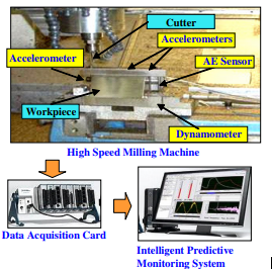
\includegraphics{img/CNC}
    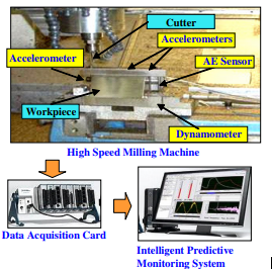
\includegraphics[scale=1]{img/CNC}
    \caption{Monitoramento das condições da ferramenta no processo de fresamento em alta velocidade}
\end{figure}

\begin{figure}[h]
  \centering
  \mbox{%
    \subfigure[Desgaste da ferramenta (cutter1).]{\label{avr-prgmem}%
      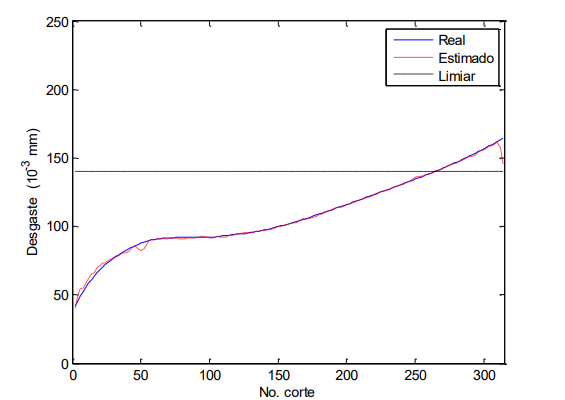
\includegraphics[scale=.4]{img/d1}}\qquad
    \subfigure[RUL da ferramenta (cutter1).]{\label{avr-datamem}%
      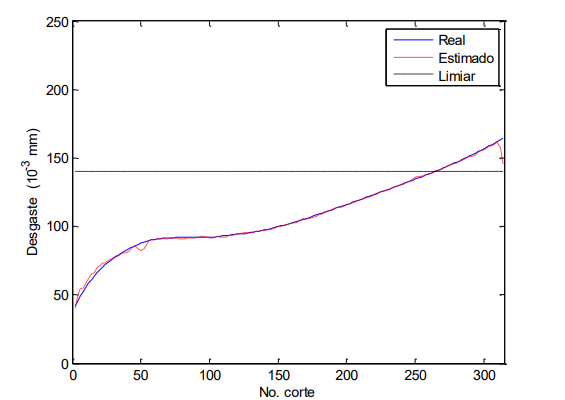
\includegraphics[scale=.4]{img/d1}}
    }
  \caption{Analise Cutter 1 \cite{inacioprognostico}}
  \label{avr-memmap}
\end{figure}


Nas figuras 2.2(a), 2.3(a), 2.4(a) podemos ver a comparação entre o desgaste real e o desgaste obtido pelo Prognostico de Falhas.


\begin{figure}[h]
  \centering
  \mbox{%
    \subfigure[Desgaste da ferramenta (cutter4).]{\label{avr-prgmem}%
      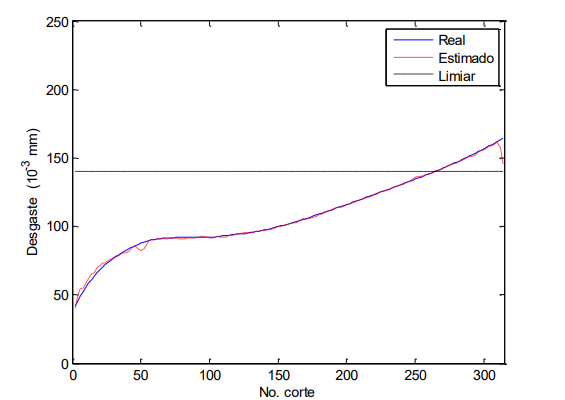
\includegraphics[scale=.4]{img/d1}}\qquad
    \subfigure[RUL da ferramenta (cutter4).]{\label{avr-datamem}%
      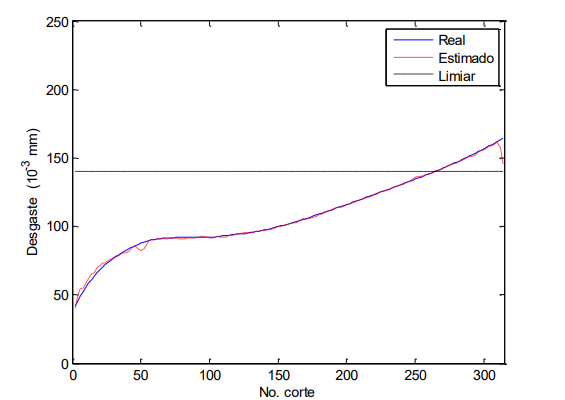
\includegraphics[scale=.4]{img/d1}}
    }
  \caption{Analise Cutter 4 \cite{inacioprognostico}}
  \label{avr-memmap}
\end{figure}

\begin{figure}[h]
  \centering
  \mbox{%
    \subfigure[Desgaste da ferramenta (cutter6).]{\label{avr-prgmem}%
      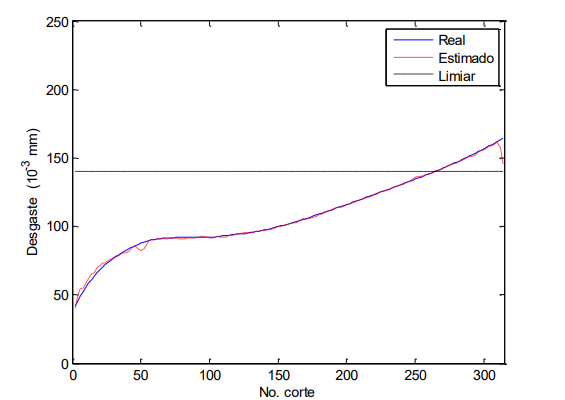
\includegraphics[scale=.4]{img/d1}}\qquad
    \subfigure[RUL da ferramenta (cutter6).]{\label{avr-datamem}%
      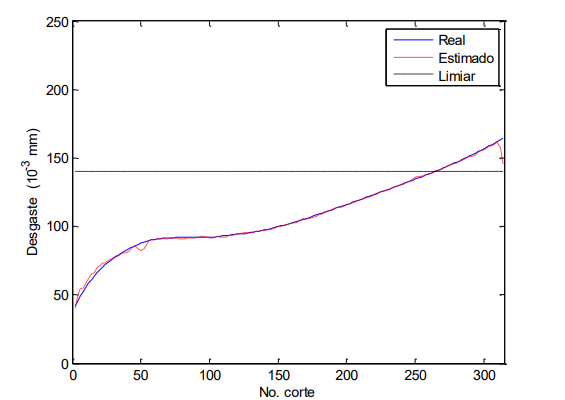
\includegraphics[scale=.4]{img/d1}}
    }
  \caption{Analise Cutter 6 \cite{inacioprognostico}}
  \label{avr-memmap}
\end{figure}
%\subsection{Tipos de Seleção de Prognósticos}

\subsection{Redes Neurais}
\subsection{Sistemas Nebulosos}
\subsection{Filtros de Partículas}

\newpage
\section{Extração de características}

Extração de características consiste em obter características especificas com base em dados observados.  O método consiste em decompor os dados já obtidos, em dados que relevantes para manter a integridade da máquina CNC, se utilizando de algoritmos \cite{liao2014discovering}.

Diversas características de domínio estatístico, frequência e tempo-frequência podem ser extraídas, desses domínios existem quatro características estatísticas mais comuns a serem extraídas e consideradas relevantes, sendo elas, Valor médio, raiz quadrada média (RMS), variância e curtose. Cada domínio pode mostrar outra visão do estado máquina \cite{wang2015enhanced}.

\begin{figure}[h]
    \centering
    %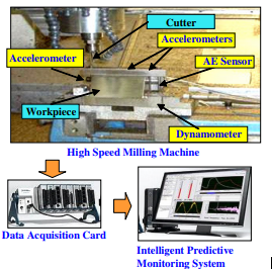
\includegraphics{img/CNC}
    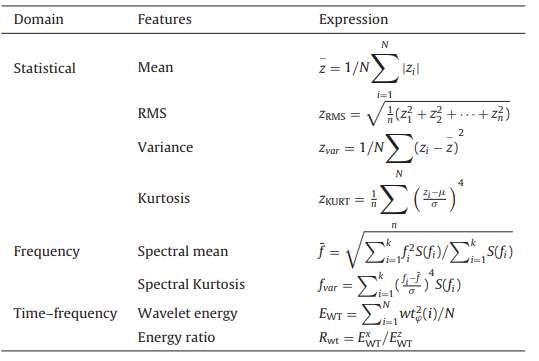
\includegraphics[scale=0.7]{img/tablect}
    \caption{Características separados por domínio \cite{wang2015enhanced} Temporario vou refazer a tabela}
\end{figure}

Em \cite{Li2009} podemos ver que a partir das características de força, foi possível se obter outras 16 caracteristicas principais usando métodos estatísticos, mostradas na Tabela 2.1.

\begin{table}[ht]
    \caption{Características Extraidas dos Sinais de Força.}
    {\centering
    \begin{tabular}{ll} \toprule
    \emph{Nº} & \emph{Característica}\\ \midrule
   1 & Erro Residual \\
2 & Diferença de primeira ordem \\
3 & Diferença de segunda ordem \\
4 & Nível Máximo de Força \\
5 & Amplitude Total da Força do Corte \\
6 & Combinação  \\
7 & mudanças de força incremental combinadas \\
8 & Desvio padrão dos componentes de força na ferramenta zona de ruptura \\
9 & Soma dos Quadrados de Erros residuais \\
10 & Taxa de pico das forças de corte \\
11 & Potência Harmônica Total \\
12 & Força Média \\
13 & Força Variável \\
14 & Desvio padrão \\
15 & Inclinação \\
16 & Curtose \\
 \bottomrule
    \end{tabular}\par
    }
\end{table}

\newpage
\section{Seleção de características}
Dado que um banco de dados, podemos ter um conjunto muito grande de dados presentes nele, muitas vezes esse conjunto possui dado que não são relevantes para o estudo a ser feito, sendo assim necessário uma seleção de tais dados. 

Após o reconhecimento dos dados presentes em tal banco de dado é feita uma extração de características, como mostrado na seção anterior. Após isso é possível que haja muitas características irrelevantes ou desnecessárias, sendo assim é necessário uma seleção de características de forma que após ela, as características selecionadas possam ser usadas para se obter o melhor resultado esperado do estudo a ser feito.

Na seleção de características, a seleção de um subconjunto de características relevantes é necessária para o estabelecer qual modelo de correlação é esperado, de forma que minimize o custo computacional \cite{Li2009}.


%\subsection{Tipos de Seleção de Características}
\subsection{Algoritmos Genéticos}
\subsection{Correlação Cruzada}